% Options for packages loaded elsewhere
\PassOptionsToPackage{unicode}{hyperref}
\PassOptionsToPackage{hyphens}{url}
\PassOptionsToPackage{dvipsnames,svgnames,x11names}{xcolor}
%
\documentclass[
]{article}

\usepackage{amsmath,amssymb}
\usepackage{iftex}
\ifPDFTeX
  \usepackage[T1]{fontenc}
  \usepackage[utf8]{inputenc}
  \usepackage{textcomp} % provide euro and other symbols
\else % if luatex or xetex
  \usepackage{unicode-math}
  \defaultfontfeatures{Scale=MatchLowercase}
  \defaultfontfeatures[\rmfamily]{Ligatures=TeX,Scale=1}
\fi
\usepackage{lmodern}
\ifPDFTeX\else  
    % xetex/luatex font selection
\fi
% Use upquote if available, for straight quotes in verbatim environments
\IfFileExists{upquote.sty}{\usepackage{upquote}}{}
\IfFileExists{microtype.sty}{% use microtype if available
  \usepackage[]{microtype}
  \UseMicrotypeSet[protrusion]{basicmath} % disable protrusion for tt fonts
}{}
\makeatletter
\@ifundefined{KOMAClassName}{% if non-KOMA class
  \IfFileExists{parskip.sty}{%
    \usepackage{parskip}
  }{% else
    \setlength{\parindent}{0pt}
    \setlength{\parskip}{6pt plus 2pt minus 1pt}}
}{% if KOMA class
  \KOMAoptions{parskip=half}}
\makeatother
\usepackage{xcolor}
\usepackage[margin=1in]{geometry}
\setlength{\emergencystretch}{3em} % prevent overfull lines
\setcounter{secnumdepth}{5}
% Make \paragraph and \subparagraph free-standing
\makeatletter
\ifx\paragraph\undefined\else
  \let\oldparagraph\paragraph
  \renewcommand{\paragraph}{
    \@ifstar
      \xxxParagraphStar
      \xxxParagraphNoStar
  }
  \newcommand{\xxxParagraphStar}[1]{\oldparagraph*{#1}\mbox{}}
  \newcommand{\xxxParagraphNoStar}[1]{\oldparagraph{#1}\mbox{}}
\fi
\ifx\subparagraph\undefined\else
  \let\oldsubparagraph\subparagraph
  \renewcommand{\subparagraph}{
    \@ifstar
      \xxxSubParagraphStar
      \xxxSubParagraphNoStar
  }
  \newcommand{\xxxSubParagraphStar}[1]{\oldsubparagraph*{#1}\mbox{}}
  \newcommand{\xxxSubParagraphNoStar}[1]{\oldsubparagraph{#1}\mbox{}}
\fi
\makeatother


\providecommand{\tightlist}{%
  \setlength{\itemsep}{0pt}\setlength{\parskip}{0pt}}\usepackage{longtable,booktabs,array}
\usepackage{calc} % for calculating minipage widths
% Correct order of tables after \paragraph or \subparagraph
\usepackage{etoolbox}
\makeatletter
\patchcmd\longtable{\par}{\if@noskipsec\mbox{}\fi\par}{}{}
\makeatother
% Allow footnotes in longtable head/foot
\IfFileExists{footnotehyper.sty}{\usepackage{footnotehyper}}{\usepackage{footnote}}
\makesavenoteenv{longtable}
\usepackage{graphicx}
\makeatletter
\newsavebox\pandoc@box
\newcommand*\pandocbounded[1]{% scales image to fit in text height/width
  \sbox\pandoc@box{#1}%
  \Gscale@div\@tempa{\textheight}{\dimexpr\ht\pandoc@box+\dp\pandoc@box\relax}%
  \Gscale@div\@tempb{\linewidth}{\wd\pandoc@box}%
  \ifdim\@tempb\p@<\@tempa\p@\let\@tempa\@tempb\fi% select the smaller of both
  \ifdim\@tempa\p@<\p@\scalebox{\@tempa}{\usebox\pandoc@box}%
  \else\usebox{\pandoc@box}%
  \fi%
}
% Set default figure placement to htbp
\def\fps@figure{htbp}
\makeatother

\usepackage{svg}
\makeatletter
\@ifpackageloaded{caption}{}{\usepackage{caption}}
\AtBeginDocument{%
\ifdefined\contentsname
  \renewcommand*\contentsname{Table of contents}
\else
  \newcommand\contentsname{Table of contents}
\fi
\ifdefined\listfigurename
  \renewcommand*\listfigurename{List of Figures}
\else
  \newcommand\listfigurename{List of Figures}
\fi
\ifdefined\listtablename
  \renewcommand*\listtablename{List of Tables}
\else
  \newcommand\listtablename{List of Tables}
\fi
\ifdefined\figurename
  \renewcommand*\figurename{Figure}
\else
  \newcommand\figurename{Figure}
\fi
\ifdefined\tablename
  \renewcommand*\tablename{Table}
\else
  \newcommand\tablename{Table}
\fi
}
\@ifpackageloaded{float}{}{\usepackage{float}}
\floatstyle{ruled}
\@ifundefined{c@chapter}{\newfloat{codelisting}{h}{lop}}{\newfloat{codelisting}{h}{lop}[chapter]}
\floatname{codelisting}{Listing}
\newcommand*\listoflistings{\listof{codelisting}{List of Listings}}
\makeatother
\makeatletter
\makeatother
\makeatletter
\@ifpackageloaded{caption}{}{\usepackage{caption}}
\@ifpackageloaded{subcaption}{}{\usepackage{subcaption}}
\makeatother

\usepackage[]{biblatex}
\addbibresource{references.bib}
\usepackage{bookmark}

\IfFileExists{xurl.sty}{\usepackage{xurl}}{} % add URL line breaks if available
\urlstyle{same} % disable monospaced font for URLs
\hypersetup{
  pdftitle={Tool Choice drastically Impacts CRISPR Spacer-Protospacer Detection},
  pdfauthor={Uri Neri*1; Antonio Pedro Camargo1; Brian Bushnell1; Simon Roux1},
  colorlinks=true,
  linkcolor={blue},
  filecolor={Maroon},
  citecolor={Blue},
  urlcolor={Blue},
  pdfcreator={LaTeX via pandoc}}


\title{Tool Choice drastically Impacts CRISPR Spacer-Protospacer
Detection}
\author{Uri Neri*\textsuperscript{1} \and Antonio Pedro
Camargo\textsuperscript{1} \and Brian
Bushnell\textsuperscript{1} \and Simon Roux\textsuperscript{1}}
\date{}

\begin{document}
\maketitle


1: DOE Joint Genome Institute, Berkeley, CA, USA\\
* Uri Neri (uneri@lbl.gov)

\section{Abstract}\label{sec-abstract}

CRISPR (Clustered Regularly Interspaced Short Palindromic Repeats)
systems are a fundamental defense mechanism in prokaryotes, where short
sequences called spacers are stored in the host genome to recognize and
target exogenous genetic elements. Viromics, the study of viral
communities in environmental samples, relies heavily on identifying
these spacer-target interactions to understand host-virus relationships.
However, the choice of sequence search tool to identify putative spacer
targets is often overlooked, leading to an unknown impact of downstream
inferences in virus-host analysis. Here, we utilize simulated and real
datasets to compare popular sequence alignment and search tools,
revealing critical differences in their ability to detect multiple
matches and handle varying degrees of sequence identity between spacers
and potential targets. Finally, we provide general guidelines that may
inform future research regarding matching, which is a common practice in
studying the complex nature of host-MGE interactions.

\section{Introduction}\label{sec-introduction}

CRISPR (clustered regularly interspaced short palindromic repeats)
systems play a vital role in prokaryotic defense against mobile genetic
elements, including viruses, plasmids, and other autonomous genetic
elements \autocite{Mojica_2005,CRISPR_review}. These systems are
organized as arrays in the bacteria or archaea genome, where short
sequences called spacers are interspersed between repeated sequences.
The spacer sequences within these arrays guide the targeting of invasive
genetic elements, allowing for specific defense against these threats
\autocite{CRISPR_classification}. The corresponding locus on the virus
genome where the spacer complements is termed ``protospacer''. The
analysis of spacer-protospacer pairs is essential in understanding the
complex interactions between hosts and MGEs
\autocite{Edwards2015_phage_host}.

The identification of genuine host-MGE interactions through
spacer-protospacer matching presents unique challenges due to the
dynamic nature of these relationships and the complexity of sequence
evolution. While matches between spacers and protospacers are often
interpreted as evidence of interaction, various biological and technical
factors can complicate this interpretation
\autocite{Edwards2015_phage_host,soto_perez_crispr_2019}.

Several key scenarios can lead to false positive assignments in
spacer-protospacer matching. Low complexity sequences can create
spurious matches between simple repeat regions (albeit these can be
mitigated through complexity filtering via Shannon entropy or DUST).
Another type of potential false positives are highly conserved sequences
shared by unrelated MGEs, potentially resulting from horizontal gene
transfer between MGEs. The horizontal transfer of CRISPR arrays
themselves on mobile elements further requires careful examination of
array genomic context (regions outside the CRISPR loci) and phylogenetic
analysis. Self-targeting events, where matches occur against the host
genome rather than MGEs, necessitate comparison against host genome
databases and analysis of targeting context. Finally, historical
acquisition events may not reflect current interactions, requiring
consideration of phylogenetic dating, evolution rates and the effects of
the protospacers being under selective pressure to mutate (which may
reduce the MGE susceptibility to deterioration by the CRISPR system).
This is further complicated by the fact that increasing the allowed
distance between sequences directly increases the likelihood of
considering sequences similar or related to each other.

False negatives present another challenge in spacer-protospacer
matching, particularly when dealing with large databases of potential
targets. Many alignment and search tools default to reporting only the
best matches or the first matches that pass a given threshold for a
given query or HSP. This may result in potentially missing additional
legitimate matches. Unfortunately, different tools also handle ambiguous
or secondary alignments differently: they may be reported, reported up
to a number or based on relative alignment quality, or omitted.
Similarly, cases where a query sequence has multiple matches in
different reference sequences are not handled uniformly across tools.
This limitation becomes increasingly problematic as databases grow
larger and more diverse, a single spacer might match (implying a
targeting) multiple related MGEs.

Yet despite these variations, the choice of spacer-to-protospacer search
or alignment tool is often not deeply considered. Presently, the common
option for this task, popularized by Edwards et al and Biswas et al
\autocite{Edwards2015_phage_host,Biswas2013}, uses BLASTn
\autocite{Altschul1990_blast} with parameters adjusted for short input
sequences. However for most bioinformatic tools, the exact workflow
design and parameter choice can impact the outcome, including in
sequence analysis. The importance of proper tool usage and parameter
interpretation is highlighted by historical examples in bioinformatics.
A striking example is the work of Shah et al, \textcite{Shah2018}, in
which they report how certain misunderstandings of BLAST's
\texttt{-max\_target\_seqs} parameter may lead to incorrect assumptions
about result completeness, potentially impacting published analyses.
Albeit this was later clarified by Madden et al., \autocite{Madden2018}
(of the blast development team) as an unfortunate combination of a
software bug (that were since patched) affecting rare cases, and
misconceptions regarding the process BLAST+ uses for tie-breaking
(alignments of equal plausibility), and finally a consideration
regarding composition base scoring. Apart from the patched bug, the main
outcome of this correspondence led to more explicit details in blast
documentation (specifically the appendix ``Outline of the BLAST
process''). Still, this highlights that misconceptions about the
expected exhaustiveness of tools' result-reporting can also lead to
incorrect assumptions about the outcome of an analysis. In practice,
most bioinformatic tools use various heuristics and optimizations,
typically designed with specific use cases in mind. For example, most
short-read mappers assume the reference to be the output of a singular
assembly - which would imply the reference does not contain extremely
redundant copies of the same loci, or a limited number of very similar
sequences (e.g.~strain variants, alternative splice variants), and this
assumption impacts the way read mapping is computed and results are
reported.

The choice of tool and its parameters can significantly impact the
detection of these multiple matches, with some tools prioritizing speed
over completeness by limiting the number of reported matches, or by
other internal heuristics such as seed sequence selection from high
occurring sequences being penalized. This trade-off between sensitivity
and computational efficiency is especially important to consider as most
available tools were designed for different tasks than
spacer-protospacer matching (e.g.~expression analysis, homology
detection, and variant calling), and under different assumptions (such
as reference and query sequence size and database size or the nature of
the reference source: from a single isolate or metagenomic sample rather
than from aggregation of sequences from different sources).

Another potential consideration is the computational resources
requirements. Memory, storage, and availability of CPU cores are factors
differing between tools. Parameter choice may also impact these factors
considerably, with certain tools offering tunable parameters to
trade-off between sensitivity and computational efficiency. In recent
years, spacer database size has been rapidly increasing - from 366,799
unique spacers in 2017 \autocite{Shmakov_2017} to 1,173,006 unique
spacers reported in 2021 \autocite{Dion_2021} to 3,835,942 unique
spacers in 2023 \autocite{camargo_img_vr4_2023}. Similarly, public virus
and MGE databases are growing rapidly, with large contributions from
metagenomic samples resulting in routine fold increases in the number of
predicted viral contigs \autocite{camargo_img_vr4_2023}. Most tools
require more resources as the size of the database grows, and as this
trend continues, certain workflows and tools may become prohibitively
expensive to run in a reasonable time frame.

\section{Methods}\label{sec-methods}

\subsection{Tool Selection}\label{sec-tool-selection}

We evaluated several widely-used sequence alignment and search tools,
alongside an implementation of basic string containment. The tools were
selected based on their availability and historical use, and were chosen
to span a range of different algorithmic approaches. It is important to
note that these tools were not specifically designed for
spacer-protospacer matching, but rather for more general sequence search
tasks (mmseqs2, blastn-short and lexicmap), or alignment/mapping of
short reads to reference genomes (bowtie1, bowtie2, minimap2, nucmer,
bbmap-skimmer, strobealign). Additionally, our focus here is
specifically on spacer-protospacer matching, and so we did not evaluate
general host-prediction tools (even those that may perform
spacer-protospacer matching), like SpacePHARER \autocite{Zhang_2021} or
iPHoP \autocite{Roux2023_iphop}, which may perform additional analyses
based on prior additional information, such as evaluating the LCA from
multiple spacer-protospacer matches.

\begin{longtable}[]{@{}
  >{\raggedright\arraybackslash}p{(\linewidth - 6\tabcolsep) * \real{0.2000}}
  >{\centering\arraybackslash}p{(\linewidth - 6\tabcolsep) * \real{0.2444}}
  >{\centering\arraybackslash}p{(\linewidth - 6\tabcolsep) * \real{0.3778}}
  >{\raggedright\arraybackslash}p{(\linewidth - 6\tabcolsep) * \real{0.1778}}@{}}
\caption{Evaluated Tools and Their Characteristics. \emph{Indexing:
``\emph{Optional}'' - A persistent index can be generated (and used
across multiple mapping/alignment runs) but a one-off command can also
do this `on the fly'. }''Yes''* - A precomputed index is required,
\emph{``No''} - Indexing or building the database is not required. All
tools were run with default parameters unless otherwise specified. As a
general rule, parameters for each tool were chosen to maximize
sensitivity or avoid limiting the ability to detect multiple matches.
For more details about the exact configuration and version of each tool,
see the code availability below or supplementary table
1.}\label{tbl-tools}\tabularnewline
\toprule\noalign{}
\begin{minipage}[b]{\linewidth}\raggedright
Aligner
\end{minipage} & \begin{minipage}[b]{\linewidth}\centering
Indexing*
\end{minipage} & \begin{minipage}[b]{\linewidth}\centering
Publication Year
\end{minipage} & \begin{minipage}[b]{\linewidth}\raggedright
Notes
\end{minipage} \\
\midrule\noalign{}
\endfirsthead
\toprule\noalign{}
\begin{minipage}[b]{\linewidth}\raggedright
Aligner
\end{minipage} & \begin{minipage}[b]{\linewidth}\centering
Indexing*
\end{minipage} & \begin{minipage}[b]{\linewidth}\centering
Publication Year
\end{minipage} & \begin{minipage}[b]{\linewidth}\raggedright
Notes
\end{minipage} \\
\midrule\noalign{}
\endhead
\bottomrule\noalign{}
\endlastfoot
\href{https://github.com/BenLangmead/bowtie}{Bowtie1} & Yes & 2009 &
Last updated 2017, optimized for short sequences (25-50 bp, max 1kbp) \\
\href{https://github.com/BenLangmead/bowtie2}{Bowtie2} & Yes & 2012 & FM
Index, supports longer reads (\textgreater50bp) than v1. \\
\href{https://github.com/lh3/minimap2}{Minimap2} & Optional & 2018 &
Versatile, supports various sequence types \\
\href{https://sourceforge.net/projects/bbmap/}{BBMap-skimmer} & Optional
& 2014 & Part of BBTools suite \\
\href{https://github.com/ksahlin/StrobeAlign}{StrobeAlign} & Yes & 2022
& strobemer-based indexing. \\
\href{https://blast.ncbi.nlm.nih.gov/doc/blast-help/downloadblastdata.html}{BLAST+}
& Optional & 2009 & BLASTN-short is a mode (task parameter), optimized
for short sequences. \\
\href{https://github.com/soedinglab/MMseqs2}{MMseqs2} & Optional & 2017
& Fast protein/nucleotide search \\
\href{https://github.com/apcamargo/spacer-containment}{spacer-containment}
& No & - & Simple string containment. FASTA parsing with needletail,
parallel processing with rayon, and string matching with
memchr::memmem::Finder \\
\href{https://github.com/mummer4/mummer}{mummer4} & Optional & 2005 &
Fast protein/nucleotide search \\
\href{https://github.com/shenwei356/LexicMap}{LexicMap} & Yes & 2024 &
\textbf{Preprint} - Highly scalable, designed for fast querying of
genes, genomes and long reads (\textgreater100bp) \\
\end{longtable}

\subsection{Data Generation and
acquisition}\label{data-generation-and-acquisition}

\begin{longtable}[]{@{}
  >{\raggedright\arraybackslash}p{(\linewidth - 4\tabcolsep) * \real{0.1047}}
  >{\raggedright\arraybackslash}p{(\linewidth - 4\tabcolsep) * \real{0.3488}}
  >{\raggedright\arraybackslash}p{(\linewidth - 4\tabcolsep) * \real{0.5465}}@{}}
\caption{Dataset characteristics. Target is interchangeable with
``contig''.}\label{tbl-datasets}\tabularnewline
\toprule\noalign{}
\begin{minipage}[b]{\linewidth}\raggedright
Dataset
\end{minipage} & \begin{minipage}[b]{\linewidth}\raggedright
Synthetic - random sequences
\end{minipage} & \begin{minipage}[b]{\linewidth}\raggedright
IMG/VR4 (v1.1) - high confidence viral contigs
\end{minipage} \\
\midrule\noalign{}
\endfirsthead
\toprule\noalign{}
\begin{minipage}[b]{\linewidth}\raggedright
Dataset
\end{minipage} & \begin{minipage}[b]{\linewidth}\raggedright
Synthetic - random sequences
\end{minipage} & \begin{minipage}[b]{\linewidth}\raggedright
IMG/VR4 (v1.1) - high confidence viral contigs
\end{minipage} \\
\midrule\noalign{}
\endhead
\bottomrule\noalign{}
\endlastfoot
Spacer Sequence Count & 9,020 & 3,835,942 \\
Total Spacer size (bp) & 618,663 & 132,094,902 \\
Spacer Length Range & 18 - 120 & 25 - 100 \\
Spacer GC\% & 50 & 46.73 \\
Spacer Median length & 68.6 & 34.4 \\
Target Length Range & 1,501 - 200,000 & 165 - 2,473,870 \\
Target GC\% & 50 & 44.45 \\
Target Median Length & 100,831.50 & 7664 \\
Target Sequence Count & 320,000 & 5,465,076 \\
Target size (bp) & 32,266,068,302 & 79,049,118,084 \\
\end{longtable}

\subsection{Synthetic dataset}\label{synthetic-dataset}

In order to examine each tool's performance on diverse spacer-to-target
matches scenario (i.e.~different number of match, similarity between
spacer and target, etc), we created a simplistic command-line interface
Python script automating the simulation of spacer-protospacer pairs
given a set of parameters (see code and data availability). These
parameters include target contig length, GC content, spacer length,
number of occurrences in the target(s), range of mismatches, reverse
complement frequency. This allows for fine grain control over the
simulated spacer and target sequences, while recording the ground truth
for later validation. See supplementary figure 1 for a visual
representation of the data generation workflow.

\subsection{Real datasets}\label{real-datasets}

To evaluate the same tools in a ``real-life'' scenario, We used the
predicted viral contigs and CRISPR spacers from IMG/VR4
\autocite{camargo_img_vr4_2023}. IMG/VR4 was chosen for several reasons:
1) it is one of the most comprehensive databases of uncultured phage and
viral genomes, and 2) the associated CRISPR database contains a large
number of CRISPR spacer data from various genomes and metagenomes, 3)
the original database released included an existing attempt at
spacer-protospacer matching using one of the tools evaluated (blastn,
albeit with different parameters, namely the ``--max-target-seqs''),
allowing for a direct comparison to historical results. Briefly, the
viral contigs in IMG/VR4 are predicted using a combination of tools
(primarily genomad \autocite{camargo_genomad_2024}) supplemented with
existing databases such as NCBI's RefSeq and GenBank, while the CRISPR
spacers were compiled from previously predicted CRISPR arrays identified
in IMG/M genomes and metagenomes (primarily via piler-cr
\autocite{edgar_piler_cr_2007} and CRT \autocite{bland_crt_2007}). For
more information, please refer to the IMG/VR4 paper
\autocite{camargo_img_vr4_2023}.

\subsection{Alignment and Recalculation of
Mismatches}\label{sec-alignment-recalc}

For comparing alignments across tools, we used the Levenshtein distance
\autocite{levenshtein1966} (a.k.a edit distance) as our main scoring
metric. For any two sequences, this metric sums both substitutions and
gaps (i.e.~insertions and deletions) into a single value. This choice
was made to ensure consistent comparison across tools that may handle
gaps differently, and because in the context of CRISPR-based defense,
both substitutions and gaps can affect the efficiency of target
recognition.

To ensure consistent mismatch calculation across tools, we realigned all
reported matches using parasail \autocite{Daily2016_parasail},
specifically the \texttt{nw\_stats\_scan} i.e.~Needleman-Wunsch global
alignment with gap opening and extension penalties of 10, and a scoring
matrix of \texttt{nuc44}. This allowed us to calculate edit distances
independently of tool-specific scoring schemes, verify the reported
matches and their orientations, and generate standardized alignment
visualizations for manual comparison.

\subsection{Performance definition and
calculation}\label{sec-performance-calc}

We defined true and false positives/negatives differently for synthetic
and real datasets. For synthetic datasets, sequences were generated
following pre-planned insertion patterns with known coordinates,
strands, and number of mismatches. While analyzing 7,638,511 pre-planned
spacer occurrences, we discovered that some sequences could align at
unplanned locations while still meeting our mismatch threshold (≤3). To
ensure accuracy, we recalculated all alignments and filtered out
sequences with extracted contig regions longer than 130bp (120bp being
the maximum spacer length). After this validation, we identified 999,916
additional valid alignments (13 with 0 mismatches, 68,612 with 1
mismatch, 224,044 with 2 mismatches, and 707,247 with 3 mismatches),
demonstrating that with short sequences, the number of potential
spurious alignments increases substantially with the allowed mismatch
threshold. Given their validated alignment scores, we included both
pre-planned and these additional alignments in our positive set. For
real data (IMG VR4), the positive set comprised all alignments from all
tools that met the specified threshold criteria. In both cases, we
calculated standard performance metric:

Recall = true positives / (true positives + false negatives)

where true positives are matches found by a tool that exist in the
positive set, false positives are matches reported by a tool that do not
exist in the positive set, and false negatives are matches in the
positive set that were not found by the tool. We note that in this
context, ``true negative'' (i.e., a false alignment a tool did not
report) does not represent a meaningful metric.

\subsection{Benchmarking framework}\label{sec-benchmark}

\subsection{Computational Resource and runtime
tracking}\label{sec-resource-tracking}

While we have made the runtime and resource (memory and storage usage)
data available, the primary focus of this study was to evaluate the
ability of each tool to accurately identify spacer-protospacer matches,
rather than their computational performance. However, as resource usage
may become a limiting factor in the future (with the advent and
accumulation of metagenomic sequence data), we designed the benchmark to
automatically log several usage metrics.

For the synthetic data, we used hyperfine
\autocite{Peter_hyperfine_2023} to track runtime and resource usage,
with a maximum of 5 runs for each tool. For the real data, we used
SLURM's built-in accounting system for cluster-based runs
(\texttt{sacct}) via a custom script (pyseff.py)\autocite{pyseff}. For
each tool, several metrics were recorded, including wall clock time,
Peak memory usage, CPU utilization, I/O operations (see supplementary
figure 1 for an overview of the synthetic data workflow). Memory
efficiency was calculated as the ratio of the peak memory usage divided
by the total allocated memory, and it is important to note that certain
tools would identify available memory and utilize all of it, while other
tools would utilize it in a deterministic manner given input size,
parameters, threads, batch size, etc. This can also affect the overall
runtime for different tools, making it difficult to directly compare the
scaling efficiency of different tools. Additionally, the runtime
reported is not the actual runtime of the tool, but rather the runtime
of the SLURM job. While most tools were run as a single job, some tools
(notably blastn-short) failed to complete given our maximum available
resources (either due to time or memory constraints), and were instead
run as multiple jobs, on different subsets of the data. As such, the
runtime reported for these tools is the sum of the runtime of all their
jobs.

\subsection{Versioning and Reproducibility}\label{sec-reproducibility}

All tools were installed and managed using conda \autocite{conda} (via
the mamba \autocite{mamba} package manager) in isolated environments.
Each tool was installed in a separate environment to prevent dependency
conflicts and ensure reproducibility. Environment activation time was
excluded from performance measurements to focus on actual tool runtime.

The exact versions and configurations of all tools were recorded in
environment files, allowing for exact replication of our testing
environment. All benchmarks were performed on identical hardware
configurations to ensure fair comparison.

\subsection{Extensibility}\label{extensibility}

The framework is designed to be expandable through the integration of
new tools. Each tool/software configuration is saved as a separate JSON
file, which includes the exact commands and conda/mamba environment it
uses. This configuration files can use placeholder variables which the
main benchmarking script replaces with user choices during execution
(such as \{threads\}, \{contigs\_file\}, \{spacers\_file\},
\{output\_dir\}, and \{results\_dir\}). A new JSON file can be added
manually or via bench.utils.tool\_commands:add\_tool function in a semi
automated method.

\section{Results}\label{results}

\subsection{Performance as a function of mismatch
threshold}\label{sec-mismatch-performance}

\begin{figure}[H]

\centering{

\pandocbounded{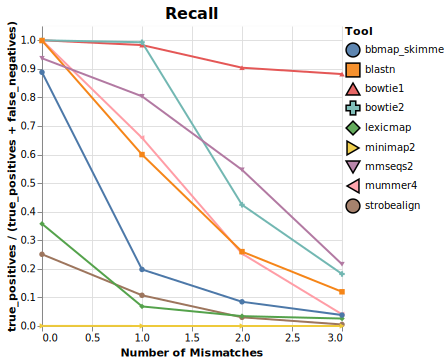
\includegraphics[keepaspectratio]{index_files/mediabag/figures/main/tool_performance_by_mismatches.pdf}}

}

\caption{\label{fig-tool-performance}Performance of each tool as a
function of mismatch threshold. The horizontal axis shows the number of
allowed mismatches, while the vertical axis represents the mean
detection fraction (0-1) aggregated across all spacer-contig pairs at a
given mismatch threshold. Each color and shape indicates a different
tool plot (shapes connected by lines for interpolation) Panel B shows
the performance of the tools on the IMG/VR4 dataset, while panel A shows
the performance of the tools on the synthetic dataset.}

\end{figure}%

First we investigated potential tradeoffs and effects of the total edit
distance (henceforth, interchangeable with mismatches) on the observed
recall metric of the tools. Generally, the detection rate of each tool
decreases as mismatch thresholds increase. Additionally, no single tool
was able to identify all spacer occurrences, although at 0 mismatches
the recall of bowtie1, bowtie2, blastn and mummer4 is approximately 0.99
(See supplementary table 2 for the recall values for each tool at
different mismatch thresholds). At increased allowed mismatches, the
tools showed more divergence, yet bowtie1 remained the single tool with
the most unique matches by a considerable margin
(Figure~\ref{fig-tool-performance}). Overall, the performance of the
tools is similar between the synthetic and real datasets, albeit the
overall lower sample size of the synthetic data should be considered
when interpreting the results (see \hyperref[tbl-tools]{table 1}).

\subsection{Performance as a function of query (spacer) abundance in
reference database}\label{sec-abundance-performance}

\begin{figure}[H]

\centering{

\pandocbounded{\includegraphics[keepaspectratio]{index_files/mediabag/figures/main/recall_vs_occurrences_combined.pdf}}

}

\caption{\label{fig-recall}Comparison of recall (detection rate) across
different mismatch thresholds and target abundance levels for IMG/VR v4
virus and spacer dataset. Top panel displays the subset of results with
up to 1 mismatch, and the bottom panel displays the results with up to 3
mismatches. The horizontal axis shows the number of target occurrences
on a logarithmic scale from 1 to 10\textsuperscript{4}, while the
vertical axis represents the mean detection fraction (0-1). Each color
and shape indicates a different tool plot (shapes connected by lines for
interpolation). The low-abundance region (1 - 1000 occurrences) is
binned into logarithmically-spaced bins, while the high-abundance region
(\textgreater1000 occurrences) is divided into only 3 additional bins,
as such ultra-high abundance sequences are rare. The detection fraction
is the mean detection fraction across all spacer-contig pairs at a given
mismatch threshold and target abundance level.}

\end{figure}%

We then investigated if there are any potential effects for the number
of times each protospacer sequence appears in the target set (i.e.~the
virus sequence set). For perfect matches (0 mismatches), bowtie1
demonstrates exceptional performance with recall rates consistently
above 0.99 across all occurrence frequencies (Figure 2). Mummer4,
bowtie2 and blastn all maintain a detection rate close to bowtie1. For
low-occurrence spacers (1-10 occurrences), strobealign achieves
detection rates of 95.44\% but shows a systematic decline to
approximately 20\% for spacers occurring \textgreater100 times, and
further drops below 5\% in the high occurrence range (\textgreater1000).

When allowing one mismatch, the overall detection capabilities decrease
across all tools, although Bowtie1 maintains its high performance. At up
to three mismatches, the overall recall rates for all other tools
further decrease, while Bowtie1 maintains detection rates above 97\%
throughout the occurrence spectrum.

The data shows a consistent pattern where detection rates generally
decline for spacers with very high occurrence frequencies
(\textgreater1000), though this effect becomes less pronounced as more
mismatches are permitted. Quantitatively, this decline is most evident
in tools like strobealign and bbmap-skimmer, while bowtie1 maintains its
high performance even with highly repetitive sequences. Detailed
statistics and recall curves for exact mismatch values (rather than at a
maximal value) can be found in the supplementary.

\subsection{Overall number of identified
spacer-contig}\label{sec-pairwise}

\begin{figure}[H]

\centering{

\pandocbounded{
\includegraphics[keepaspectratio]{index_files/mediabag/figures/main/tool_comaprison_matrix.pdf}}

}

\caption{\label{fig-pairwise}Tool vs Tool (pairwise) comparisons - set
intersections and differences matrixes. The value of a cell(i,j) is
number of spacer-contig pairs identified by the tool listed in row i,
which were not identified by the tool listed in the j column. Panel A
shows the results for the synthetic dataset, while panel B shows the
results for the IMG/VR4 dataset.}

\end{figure}%

The pairwise comparison of the tool results suggests
(Figure~\ref{fig-pairwise}), reinforces the observation regarding
bowtie1's unique ability to recover a maximum number of spacer matches.
Generally, it appears that, when compared to any single other tool, the
total number of contig-spacer pairs bowtie1 misses is relatively smaller
than the number of pairs the compared tool identified which were not
identified by bowtie1.

\section{Discussion}\label{discussion}

Our findings reveal that within the mismatch thresholds tested (less or
equal to 3), no single tool was able to identify all spacer occurrences.
While we observe variations across tools, the main difference appears to
be the effect of the abundance of the spacer in the target set on the
recall rate. Of specific concern is the relatively high number of
alignments missed by blastn-short, which is the common method currently
used. In this context, missing potential spacer-protospacer pairs can
significantly impact downstream conclusions, e.g.~about host range of a
given MGE. Overall, Bowtie1 presented the highest recall, although still
imperfect for non exact matches. It should be noted that bowtie1 is not
designed to identify \textgreater3 mismatches, and so a truly exhaustive
approach might be to utilize a combination of tools to increase the
recall rate, and use a post-search verification method (such as the
score recalculation performed here using parasail) to remove potential
false positives. Potentially, low complexity sequence filtering (or
masking) could be performed prior to the search.

It should be noted that experimental and analytical context may have to
be considered when deciding on a specific tool, especially in settings
where a higher level of sequence dissimilarity could be considered. On
one hand, spacer and virus databases can be expected to continue to
increase in size, and our results suggest that large-scale meta-analysis
studies (in which spacers from multiple samples are compared to a many
potential targets that may include similar or identical regions), should
favour tools with high recall, to circumvent potential reporting
limitations other tools might have. This is especially important as in
such meta-analysis, it should not be assumed the spacer and the
potential target co-occur (from the same biological sample) and though
the similarity may imply a past encounter between the ancestors of the
sequences, caution is due in inferring that the current MGE sequence is
capable of infecting the host sequence. In contrast, in experimental
designs where potential CRISPR-target pairs are constrained by prior
knowledge, tools with higher tolerance for sequence mismatches such as
bowtie2 or BLASTn may be more appropriate (e.g.~when studying known
phage-host pairs from isolates, or when investigating temporally
resolved samples (e.g.~time-series)).

Another consideration should be the source of the spacer data: spacers
sequences extracted from raw NGS data and spacers extracted from
assembled CRISPR arrays (either from assembled or long read sequencing).
Specifically, spacers from complete arrays present additional
information, namely the location and order of the spacers within the
array, and the observation they originate from the same host genome.
Notably, a recent in-depth study by Mitrofanov et al
\textcite{Mitrofanov2025}, investigating the mutational landscape of
repeats across many isolate prokaryote genomes, have identified patterns
of spacer loss based on system sub/type and location. A similar
meta-analysis of spacer mutations by Vink et al \textcite{Vink2021},
have revealed that different CRISPR subtypes exhibit varying tolerance
for mismatches within the spacer sequences, with most matched spacers
containing three or fewer mismatched nucleotides. This aligns with our
current general recommendation of using Bowtie1. Additionally, Vink et
al observed that Type I-E and Type II systems preferentially target
template strands while Type I-A, I-B, and Type III systems prefer coding
strands, emphasizing system-specific characteristics which may also
inform post-search verification methods (albeit this may require
additional information, such as the sequences orientation or coding
potential, and the CRISPR subtype of the spacer).

While our technical comparison focuses on tool performance, the
biological interpretation of identified matches also requires careful
consideration. The arms race between prokaryotes and MGEs creates a
complex landscape where simple sequence matching may not directly
translate to genuine host-parasite relationships. We identified several
scenarios that could lead to false positive assignments:

\begin{enumerate}
\def\labelenumi{\arabic{enumi}.}
\item
  \textbf{Low Complexity Sequence Matches}: Independently of the tool
  choice, low-complexity (regions with highly skewed GC content, or
  composed of many repeated sequences) can be susceptible to spurious
  matches. Low complexity regions may be present in both the virus
  target set, or in the spacer set, where some non-CRISPR repeated
  sequences may have been misclassified as such. While certain tools
  employ filters and heuristics to mitigate the effect of low complexity
  regions, a prudent procedure should include a step separated from the
  search, to specifically identify, filter or mask the spacer and virus
  sets. Dustmasker \autocite{Morgulis_2006}, or a similar tool
  (e.g.~ldust from minimap, or BBDuk from bbmap) could be used prior to
  the search.
\item
  \textbf{Common Sequence Motifs}: Some matches may correspond to highly
  conserved sequences shared across various biological systems. For
  instance, horizontal gene transfer events can lead to the spread of
  similar sequences across diverse MGEs, potentially creating spurious
  matches that don't reflect direct host-MGE interactions. An example of
  potential HGT mediated matches was described by Kosmopoulos et
  al.~2023, where a transposon-mediated transferred of a phage lysin
  gene (to the host genome) created a true sequence similarity (which
  was verified by the authors using a combination of sequencing
  technologies) \autocite{Kosmopoulos_2023}. Even if anecdotally
  observed, this suggests that an unknown number of observed ``good''
  alignments may be due to HGT, which in the absence of additional
  information, could not be ruled out as a false positive.
\item
  \textbf{Self-Targeting Events}: Some matches may represent CRISPR
  targeting of host genes \autocite{Wimmer_2020}. Previous studies
  estimated a varying amount of these actually target sequences with
  putative exogenous origin such as prophages, ranging from
  \textasciitilde50\% \autocite{Stern_2010}, to \textasciitilde80\%
  \autocite{Shmakov_2017}. In Shmakov et al., the authors estimate
  non-defence targeting is likely a rare event. So far, most
  observations of non-defence (or counter defence) molecular functions
  of CRISPRs did not directly involve the spacer sequences, but rather
  the Cas genes or related effectors. Some observed functions include
  genome remodelling and evolution, or temporal regulation of gene
  expression. For example, in \emph{Francisella novicida}, Sampson et
  al.~2013 demonstrated that certain lipoprotein production is mediated
  by a CRISPR system \autocite{Sampson_2013}.
\item
  \textbf{non-chromosomal replicon encoded CRISPRs}: Similarly to the
  potential of CRISPR systems to act in non-immune functions, in certain
  scenarios spacers may be acquired from non-MGE replicons, or be
  carried (even if partially) by mobile elements. While some types are
  known to be chromosomal, others are known to be carried entirely by
  plasmids (i.e.~both the Cas proteins and the array loci are on the
  plasmid), for example in various halophilic archaea
  \autocite{Maier_2018}. A recent study by Zhang et al
  \autocite{Zhang_2025} observed similar phenomena in the human gut
  microbiome, specifically in \emph{Bifidobacterium longum}. Another
  non-MGE targeting phenomena in archaea was described by Turgeman-Grott
  et al. \autocite{Turgeman_Grott_2018}, where inter-species spacers
  (targeting genes from related species) were demonstrated to be common
  in archaea, at least in the context of cellular mating. Another
  confounding factor is the potential of certain MGEs to target host
  genes, potentially for regulatory functions, or as counter-defense
  mechanisms\autocite{Shmakov_2023}. Shmakov et al.~2023 have identified
  widespread CRISPR-derived phage-encoded mini-arrays, which can hijack
  and interfere with their host native system.
\end{enumerate}

\subsection{Study Limitations}\label{study-limitations}

The synthetic data was generated with uniform distributions of spacer
and contig lengths and base composition (where each nucleotide is chosen
independently and at random). While the simulation scripts do allow
user-specified base composition (or use of real data via the --contigs
or --spacers parameters), real biological sequence composition is not
usually uniformly distributed, and may be biased towards certain
nucleotide frequencies, which could be region or loci specific. This can
be clearly observed comparing the spacer attributes distributions in the
synthetic and real datasets (see supplementary figure 6), and table 1.
While the simulated dataset sample size is relatively small, the high
level of control over the spacer and contig sequences allowed testing
rare or yet-unobserved scenarios, like ultra high spacer occurrence
rates. This difference in sample size and features should be considered
when interpreting the results.

Furthermore, we focused on a specific distance metric (Levenshtein
distance), thus the synthetic sequences only have substitutions
simulated into them. While insertions and deletions were not simulated,
and although these might be relatively rare in short evolutionary time,
they are still possible and could inform real and recent MGE-host
interactions (e.g an indel that does not disrupt the encoded sequence
reading frame). This could be further explored in future work, and might
affect overall tool suggestion to use bowtie1 for general-case
spacer-protospacer matching, as it is not designed with gaps in mind.
Finally, we note that tools were not tested for all possible
combinations of their available tunable parameters, and it is possible
some might be further tweaked to improve their performance. Similarly,
variation in parameters during index construction may further affect
this (e.g.~offset rate, seed selection). Similarly, not all major
versions of all tools were tested. Of specific note are MMseqs2 (where
the latest release version at the time of execution resulted in frequent
crashes, hence we used the latest commit version from github), and
Lexicmap which does not have a formal ``v1'' release at the time of
writing, and since the benchmark was run, a new minor version was
released, which is a good candidate for future testing.

\section{Conclusion}\label{conclusion}

Our comparison of spacer-protospacer search tools reveals variations in
their ability to detect unique putative CRISPR-target matches, which is
a key and common input for current host-MGE interaction tools and
studies. The main tool-derived difference we report is the ability to
detect multiple matches - most tools show a sharp decline in detection
rates as the total number of occurrences increases. This can directly
impact the downstream interpretation of microbial relationships, such as
under estimation of potential hosts-range, or over reliance on seemingly
unique matches which may actually be due to non-direct intercations
resulting from common sequence motifs or high tolerance for mismatches.
While Bowtie1 demonstrates superior performance in detecting multiple
matches under the threshold of 3 mismatches, the interpretation of
spacer-protospacer matches requires careful consideration of biological
context and potential interfering factors, especially when comparing
large databases of CRISPR spacers and potential targets collected from a
broad range of samples and ecosystems. Our findings also emphasize the
importance of recalculating alignment metrics in a tool-agnostic manner,
to ensure consistent comparison across tools. Finally, we provide
general recommendations and experimental design considerations of
potential interfering factors for future studies.

\section{Code and data availability}\label{code-and-data-availability}

All code generated for this study can be found in the git repository:
\href{http://code.jgi.doe.gov/spacersdb/spacer_matching_bench}{code.jgi.doe.gov/spacersdb/spacer\_matching\_bench}.
All raw outputs (tool results on real and synthetic datasets, the
simulated sequence files, the SLURM logs, and the hyperfine runtime
measurements) are available on Zenodo \autocite{zenodo_doi}.

\section{Acknowledgements}\label{acknowledgements}

Work conducted by the U.S. DOE Joint Genome Institute
(https://ror.org/04xm1d337) (SR, UN, APC and BB), a DOE Office of
Science User Facility, is supported by the Office of Science of the U.S.
DOE operated under Contract DE-AC02-05CH11231.

We would like to thank the following people for their helpful feedback
and suggestions: Uri Gophna and Georg Rath.


\printbibliography



\end{document}
